\section{\acrlong{ir} Methods}\label{sec:ir_methods}

In this section, we introduce the \gls{ir} methods that we will be testing.
We have chosen these methods to evaluate different ways of performing an \acrfull{ir} task.

The goal of each method is to produce a document-score vector with one score for each document in the corpus, indicating the relevance of the document compared to the query.
These scores can then be sorted in descending order to produce a ranking of the documents.

Some of the methods calculate scores for a single word at a time rather than a whole query.
In that case, we treat their score as an estimate of the probability that a document $d$ generates a specific word $w$.
To find the probability of $d$ generating a given query $q$, we take the product of the word probabilities for each word in the query $w \in q$, as the document would have to generate each word, as shown in \autoref{eq:query_prob}.

\begin{equation}\label{eq:query_prob}
	P(q|d) = \prod_{w \in q} P(w|d)
\end{equation}

\subsection{\acrlong{lda}}\label{sec:lda}
\Gls{lda} is topic model method.
The objective of topic modeling is to infer topics (collections of words) in a document set.

\begin{definition}\label{def:topic}
	\textit{A topic is a distribution over words in a corpus.}
\end{definition}

The result consists of a topic-word distribution matrix $\beta$, which for each topic gives a distribution of words belonging to said topic, and a document-topic distribution matrix $\theta$ which for each document gives a distribution of topics to which the document belongs to.

\citet{lda} introduced \gls{lda}, which has since become a staple within topic modeling.
\gls{lda} works under the assumption that documents are generated from a specific generative process, and tries to reverse engineer this process.
This generative process assumes that documents are random mixtures of latent topics and that each topic is a distribution over all the words in the corpus.

This process generates $K$ topics and $D$ documents containing $N_{d}$ words, where $d$ is a document in $D$.
The generative process has two Dirichlet distributions $Dir(\alpha)$ for the document-topic relation and $Dir(\eta)$ for the topic-word relation.

\begin{figure}[h]
	\centering
	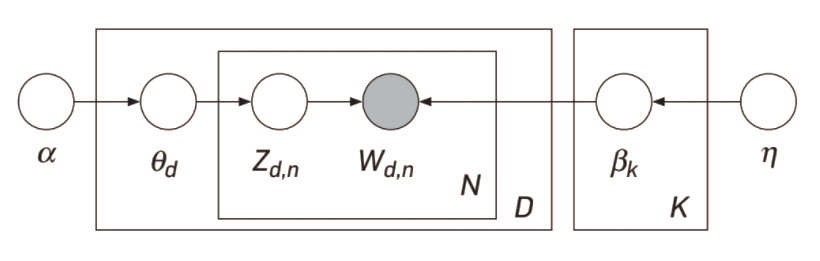
\includegraphics[width=0.5\textwidth]{figures/Smoothed_LDA.jpg}
	\caption{Plate notation for \gls{lda}. Boxes symbolize repeated processes, shaded elements are observed information. Image is from \citet{blei2012topicmodels}.}
	\label{fig:lda}
\end{figure}

From these Dirichlet distributions, we can sample two multinomial distributions: a document-topic distribution $\theta_d$ for each document $d$, and a topic-word distribution $\beta_k$ for each topic $k$.
$\theta$ and $\beta$ are stored as matrices.
These Dirichlet distributions are tuned with the hyperparameters $\alpha$ and $\eta$, which adjust the entropy of the sampled distributions.
An $\alpha$ value near 1 causes each document to be distributed over almost all topics, while an $\alpha$ value near 0 causes each document to be distributed over only a few topics.
Similarly $\eta$ will adjust how many words each topic contains.
This also has the added consequence that a high $\alpha$ will make documents appear more similar, and a high $\eta$ will make topics appear more similar.

Using $\theta$ and $\beta$, we can sample concrete topics $Z$ from documents, and concrete words $W$ from topics.
\autoref{fig:lda} gives an overview of the generative process.

\Gls{lda} has some underlying assumptions, which also explain its limitations\cite{blei2012topicmodels}:
\begin{itemize}
	\item \gls{lda} assumes ordering of words does not matter (Bag of Words).
	\item \gls{lda} assumes ordering of documents does not matter.
	\item \gls{lda} assumes that the number of topics is fixed and known.
\end{itemize}
However, many of these assumptions can be addressed through various extensions of the \gls{lda} model\cite{blei2012topicmodels}.

\subsubsection{\gls{lda}-\gls{ir}}\label{subsec:lda_ir}
\gls{lda} is not designed as an \acrlong{ir} method.
And as such, it usually gives subpar performance when applied to \gls{ir} tasks.
This is due to topic modeling working on the more abstract level of topics, rather than word frequencies as many of the other \gls{ir} methods.
However, this also gives \gls{lda} the ability to understand topics expressed in queries and do \gls{ir} based on that knowledge.

\citet{yang2009topic} defines \autoref{eq:lda-ir} for using \gls{lda} as an \gls{ir} method.
They do this based on a previous application of \gls{lda} for \gls{ir}\cite{lda-ir}.

\begin{equation}\label{eq:lda-ir}
	P(w|d, \theta, \beta) = \sum_{z \in T} P(w|z,\beta_z) P(z|d,\theta_d)
\end{equation}

The idea behind this equation is to reverse-engineer the generative process \gls{lda} uses to create the topic model, to predict the probability of a word appearing in a document given the document-topic distribution matrix $\theta$ and the topic-word distribution matrix $\beta$.
So, for each topic $z$, the probability of the word $w$ using $\beta_z$ is multiplied with the probability of that topic appearing in the document using $\theta_d$.

This is similar to the process \gls{lda} uses to generate topics, but instead of constructing topic-word distributions and document-topic distributions based on observed words, we now use these distributions and the observed words to find the probability of a word appearing in a document based on its topic distribution.
In practice, we multiply the $\theta$ and $\beta$ matrices together and get a $document \cdot word$ matrix, where each cell represents the probability of a given word appearing in a specific document w.r.t. the topic they share.
We use the term \gls{lda}-\gls{ir}, to refer to information retrieval made using \autoref{eq:lda-ir}.

\section{Language model}\label{sec:language_model}
The \gls{lda} model gets poor document retrieval performance when not used in combination with another model\cite{yang2009topic}.
In \cite{yang2009topic}, they describe various combinations of \gls{lda} and other models. 
The language model they describe is similar to a query likelihood model, which generates a probability of how likely a given document $d$ produces a given query $q$.
To calculate this probability, they find the likelihood for each word in the query by using this function:
\begin{equation}\label{eq:word_prob}
	P(w|d) = \frac{N_d}{N_d + \lambda} \cdot \frac{tf(w,d)}{N_d} + (1 - \frac{N_d}{N_d + \lambda}) \cdot \frac{tf(w,D)}{N_D}
\end{equation}

where $N_d$ is the number of word tokens in document $d$ and $tf(w,d)$ is the word frequency of word $w$ in document $d$. Likewise, $N_D$ is the total number of word tokens in the corpus $D$, and $tf(w,D)$ is the word frequency of word $w$ in the whole corpus $D$. $\lambda$ is a Dirichlet smoothing factor and is set to the average document length.
$ \frac{N_d}{N_d + \lambda} $ describes a relative term which is weighted based on $ \lambda $. If $N_d > \lambda$ the value is closer to 1 and if $ N_d < \lambda $ the value is closer to 0.
$ \frac{tf(w,d)}{N_d} $ and $\frac{tf(w,D)}{N_D}$ are the maximum likelihood estimate of $w$ appearing in a document $d$ or the corpus $D$, respectively.
\autoref{eq:word_prob} calculates the relative maximum likelihood for the word being in $ d $ and $ D $, and weighs these terms based on the document length $N_d$ compared to $\lambda$, with smaller documents weighing the corpus likelihood higher, and bigger documents weighing the document likelihood higher.

To calculate this for a given query, we take the product of the word likelihood to get the probability for $q$.

\begin{equation}\label{eq:query_prob}
	P(q|d) = \prod_{w \in q} P(w|d)
\end{equation}

\cite{yang2009topic} combine the \gls{lda} model and the language model to get information about the topic and word correlation between $q$ and $d$.

\section{PageRank}\label{sec:pagerank}
\gls{pr} is a recursive ranking algorithm, used to rank nodes in a graph.
It is based on the random surfer model, where several surfers would take $s$ amount of steps across a graph.
The number of surfers standing on a given node would be the resulting score for that node.
The \gls{pr} algorithm is defined as follows (expressed in matrix form) \cite{ClusterPageRank}.
$$ \overrightarrow{s} = \mu \widetilde{M}^T \overrightarrow{s} + \frac{(1-\mu)}{|D|} \overrightarrow{e} $$  
where $\overrightarrow{s}$ is a vector consisting of scores for each document. 
$\mu$ is the dampening factor which is set to $0.85$.
$\widetilde{M}^T$ is the adjacency matrix transposed.
$|D|$ is the number of documents.
$\overrightarrow{e}$ is a column vector where all elements are equal to 1.

We construct a graph over our documents, where edges between documents $d_i$ and $d_j$ are based on the similarity between them $sim(d_i, d_j)$.
We run the \gls{pr} algorithm for 20 iterations.
This allows us to use \gls{pr} on the graph to search for similar documents.
To construct the adjacency matrix for the graph, we apply a similarity function on each pair of document-topic distributions $\theta_{d_i}, \theta_{d_j}$, from our topic model.

We use Jensen-Shannon distance as our similarity function, which is a measure of the distance between probability distributions\cite{jensen-shannon2003}\cite{jensen-shannondis2003}.
It is calculated using the square root of the Jensen-Shannon divergence between two probability distributions and gives a score from 0 to 1.
However since Jensen-Shannon calculates difference rather than similarity, a low value means more similarity, making our similarity function:
$$sim(d_1, d_2) = 1 - JS(\theta_{d_1}, \theta_{d_2})$$

The Jensen-Shannon distance function is defined as:
$$ JS = \frac{D(p || m) + D(q || m)}{2}$$
where $p$ and $q$ are distributions and $m$ is the pointwise mean between $p$ and $q$. 
$D$ is the Kullback-Leibler divergence function.

The goal of using \gls{pr} is to get the most important documents within a specific topic and use these to yield important information during search.  


\subsection{\acrlong{tf-idf}}
\acrfull{tf-idf} is a well known \gls{ir} method that is used to find the most important words within texts.
As the name suggests, this method aims to balance the two measures: term frequency and inverse document frequency.
In our case, terms are the words left in the documents after the preprocessing phase.
For each term in the query $t \in q$, a \gls{tf-idf} score will be calculated for each document in the corpus $d \in D$.
Thus each document will have one score for each term in the query.
These scores are combined into one score for each document using \autoref{eq:query_prob}.


Term frequency describes how often a word is used within a specific document.
Inverse document frequency describes how many documents in the corpus includes the given term.
The IDF value decreases the more widely used the given term is.
The overall goal of \gls{tf-idf}, is giving a measure of how often used and unique a term is for a given document. Words that are often used in the given document, but rarely used in the corpus will have the highest \gls{tf-idf} scores.

The formula for \gls{tf-idf} can be seen in \autoref{eq:tfidf}

\begin{equation}\label{eq:tfidf}
	\text{tf-idf}(t, d, D) = \text{tf}(t, d) \cdot \text{idf}(t, D)
\end{equation}

\begin{equation}\label{eq:idf}
	\text{idf}(t,D) = log \frac{|\{d \in D\}|}{|\{d \in D : t \in d\}|}
\end{equation}
	
Where tf$(t, d)$ is the number of times a term $t$ appears in a document $d$ from the corpus $D$.

\subsection{\acrlong{bm25}}
\todo[inline]{describe goal / purpose / idea}
\gls{bm25} is a bag of words retrieval function, which is similar to \gls{tf-idf}, since it uses the inverse document frequency.
The formula for \gls{bm25} can be seen in \autoref{eq:bm25}\cite{bm25}.
\begin{equation}\label{eq:bm25}
	\text{bm25}(d, q) = \sum_{i=1}^{n}\text{idf}(q_i) \cdot \frac{\text{tf}(q_i, d) \cdot (k_1 + 1)}{\text{tf}(q_i, d) + k_1 \cdot (1 - b + b \cdot \frac{|d|}{avgdl})}
\end{equation}
where tf$(q_i)$ is the number of times the term $q_i$ appears in $d$.
$|d|$ is the number of words in d. 
$avgdl$ is the average document length from the corpus.
$b$ and $k_1$ are both hyperparameters, which are set to $0.75$ and $1.5$, respectively.

\subsection{Combining \gls{ir} Methods}
Each of the \gls{ir} methods, described in this section, has its own strengths and weaknesses.
We combine multiple of these methods, to see if they can draw upon each other's strengths and cover each other's weaknesses.
We hypothesize that combinations will be able to produce better results than each of the methods separately.

As with \citet{yang2009topic}, we combine multiple \gls{ir} methods by normalizing their document-score vectors and then either summing or multiplying them together element-wise.
This process is visualized in \autoref{fig:combine}.

\tikzstyle{process} = [circle, rounded corners, minimum width=2cm, minimum height=1cm,text centered, draw=black, fill=gray!50]
\tikzstyle{decision} = [diamond, minimum width=3cm, minimum height=1cm, text centered, draw=black, fill=green!30]

\begin{figure*}[ht]
    \centering

\begin{tikzpicture}
\matrix [matrix of nodes,row sep=0mm, set common column={2,3,4,5,7}{nodes={rectangle,draw,minimum width=3em}}, set common row={1,3} {nodes={draw=none}}, ] (O)
{
    & $D_0$ & $D_1$ & $D_2$ & $D_3$ &  & $D_n$ \\
    BM25 (b) & $S^{b}_{D_0}$ & $S^{b}_{D_1}$ & $S^{b}_{D_2}$ & $S^{b}_{D_3}$ & \dots & $S^{b}_{D_n}$  \\
    & + & + & + & + &  & +\\
    PR (p) & $S^{p}_{D_0}$ & $S^{p}_{D_1}$ & $S^{p}_{D_2}$ & $S^{p}_{D_3}$ & \dots & $S^{p}_{D_n}$\\[8mm]
    BM25+PR & $S^{b}_{D_0} + S^{p}_{D_0} $ & $S^{b}_{D_1} + S^{p}_{D_1} $ & $S^{b}_{D_2} + S^{p}_{D_2} $ & $S^{b}_{D_3} + S^{p}_{D_3} $ &  \dots & $S^{b}_{D_n} + S^{p}_{D_n} $\\
};

\foreach\x in{2,3,4,5,7}{\draw[my arrow] (O-4-\x) to (O-5-\x);}
\end{tikzpicture}
    \caption{Example of combining two \gls{ir} methods. Here \gls{bm25} and \gls{pr} are summed together by summing their document-score vectors element-wise.}
    \label{fig:combine}
\end{figure*}


Both of these options are viable and have their own benefits and drawbacks.
Summation allows documents to be ranked fairly high even if one of the combined methods produce a low score.
With multiplication, a document with average scores for each method can have a better rank than one with mostly good scores but a really low score from one of the combined \gls{ir} methods.
